\section{Introducción}
%%%%%%%%%%%%%%%%%%%%%%%%%%%%%%%%55%%%%%%%%%%%%%%%%%%%%%%%%%%%%%%%%%%%%%%%%%%%%%%%%%%%%%%%%%%%%%%%%%%%%%%%%%%%%%%%%%%%%%%%%%%%%%%%%%
% requerimientos,Hacer como una sinopsis.
%%%%%%%%%%%%%%%%%%%%%%%%%%%%%%%%%%%%%%%%%%%%%%%%%%%%%%%%%%%%%%%%%%%%%%%%%%%%%%%%%%%%%%%%%%%%%%%%%%%%%%%%%%%%%%%%%%%%%%%%%%%%%%%%%%%
Especialistas de distintos ámbitos académicos o profesionales se encuentran habitualmente en la necesidad de realizar estudios del movimiento del cuerpo humano. Esta tarea implica registrar la posición de miembros o articulaciones en el espacio y su correspondiente evolución en el tiempo.

Algunos ejemplos correspondientes a distintas áreas que ilustran estas necesidades son:

\begin{itemize}
\item A \emph{nivel asistencial}, en el área de \emph{fisioterapia}. Para realizar un seguimiento de la evolución de un paciente resulta importante en muchos casos conocer en detalle el movimiento, posición, etc. de la articulación o miembro afectado para llevar un control del mismo durante la rehabilitación y así poder determinar con mayor exactitud el estado del paciente.
\item \emph{Investigación académica en biomecánica}. Diversos proyectos se llevan a cabo en las universidades sobre esta temática, por ejemplo, en la facultad de ingeniería de la Udelar  se realizó el estudio comparativo de la patada delfín y la patada “crawl” respecto al nado de los peces por ondulación, tratando de explicar cómo la misma puede ser propulsiva. Para ello se analizaron videos de nadadores olímpicos mediante los cuales se obtuvo una secuencia temporal de las posiciones de diferentes partes del cuerpo durante varios ciclos de patada.
\item \emph{Medidas de performance en el deporte de alto nivel}. Cuando se habla de entrenamiento deportivo se hace referencia tanto a la mejora de las capacidades del atleta como a la optimización de las capacidades en función del deporte en el que se desempeña. La técnica deportiva está relacionada directamente con la optimización de estas capacidades por lo que una buena técnica garantiza el mejor aprovechamiento de las posibilidades físicas del atleta garantizando mejores resultados. Las mejores soluciones para la optimización de la técnica de un deportista consisten en el análisis de videos donde se puede estudiar en detalle cada uno de los movimientos del  mismo.
\item \emph{Animación 3D}. Probablemente el más conocido de estos ejemplos, tanto en el diseño de videojuegos como en películas, programas de televisión o comerciales muchas veces se requiere capturar el movimiento de un actor para interpretear un personaje  y que sus movimientos parezcan lo más natural posible.
\end{itemize}

En este contexto, el análisis de video  es  una  herramienta  fundamental para la recolección y estudio de datos. El seguimiento de puntos de referencia, se utiliza para el cálculo de posición y otras variables asociadas como son la velocidad, la aceleración y por ende desplazamientos. Trabajar con video, permite además estudiar secuencialmente situaciones estáticas en el tiempo. El seguimiento de dichos puntos resultaría tedioso si se hiciera manualmente por lo que resulta necesario contar con una herramienta que realice esta tarea automáticamente.

A raíz de esto, se puede definir un \emph{sistema de captura de movimiento} como un conjunto de dispositivos y software que a partir de la grabación del movimiento de una persona (o cualquier otra cosa), es capaz de trasladar dicho movimiento a un modelo digital para diferentes fines.

Los ejemplos mencionados anteriormente definen distintos casos de uso con características disímiles, de manera que la búsqueda de una solución única que abarque las necesidades particulares de todos ellos resulta compleja. Por ejemplo, en el ámbito deportivo la velocidad del movimiento es una variable importante a tomar en cuenta para desarrollar una solución, de esta variable, depende la elección tanto del sistema de adquisición como de los algoritmos más eficaces para el registro del movimiento.  De igual manera definir la portabilidad del sistema depende de si la actividad a relevar es en condiciones de laboratorio controladas o al aire libre, debido a la protección y transporte de equipos o las variaciones en las condiciones de iluminación, ruido, etc..

Al  día  de  hoy,  las  soluciones  de  software  disponibles  en  el  mercado que  podrían  asistir al especialista en su tarea, son mayormente comerciales. Las pocas alternativas de código abierto, carecen de las características necesarias al especialista o están enfocadas hacia otras áreas de aplicación. Contar con este tipo de herramientas es fundamental para las necesidades de los equipos de profesionales, cuya alternativa son productos comerciales de alto costo.

En virtud de estas necesidades este proyecto buscó \emph{relevar y caracterizar los distintos casos de uso para un sistema de captura de movimiento,  seleccionar uno que sea representativo y suficientemente general para poder realizar una aplicación básica y funcional de código abierto de análisis de video que de solución a las necesidades que se describieron, ya sea utilizando como base algún  proyecto  de  software  libre  existente,  o en su defecto, desarrollando un prototipo de software básico en su totalidad que abarque el problema en forma general, para luego estudiar extender la aplicación hacia otros casos de uso}.

Es importante resaltar la importancia de \textbf{lograr tener una primer versión del sistema de principio a fin}, con todas las etapas implementadas de forma tal de abarcar todos los procesos que la captura de movimiento implica.  Esto tiene como ventaja que se tendrá un panorama general del estado del arte de cada etapa del sistema, y en proyectos futuros se puede optimizar individualmente cada una de estas de acuerdo a las necesidades del cliente.

De acuerdo a lo planteado por el cliente y a las hipótesis que se establecieron en conjunto, se pueden realizar los siguientes supuestos:
\begin{itemize}
\item Las capturas de los pacientes se realizarán en un laboratorio con ambiente controlado:
	\begin{itemize}
		 \item La iluminación es la adecuada para realizar las  capturas correctamente
		 \item El fondo sobre el que se harán las capturas es oscuro
	\end{itemize}
\item El traje (o la ropa) que utilizará el paciente es oscuro
\item Los marcadores a detectar son esferas blancas que van colocadas sobre el cuerpo del paciente
\end{itemize}

Por otro lado, la salida del sistema debe ser la posición en el espacio de cada marcador colocado en el cuerpo del paciente, para cada instante de tiempo en la captura. Además cada marcador debe estar identificado en cada cuadro. A estos requerimientos, se le suman otros de caracter académico, como la importancia de tener una base de datos con sets de prueba y una método de evaluación de performance establecido. Estas dos cosas toman gran relevancia en etapas futuras del proyecto, ya que realizando pruebas de las nuevas implementaciones con los mismos datos que se realizaron estas y midiendo los resultados de la misma forma, se puede tener un buen punto de referencia sobre el cual comparar y poder evaluar cuanto se mejora el sistema.

En resumen, el sistema a crear pretende bajo ciertas condiciones controladas, obtener las coordenadas espaciales de un número de puntos de interés sobre un persona. Una de las formas de realizar esto es colocando a la persona un traje negro con marcadores en un ambiente con iluminación adecuada, se le filma con varias cámaras a lo largo del tiempo, se adquiere esta información en la computadora y mediante un posterior procesamiento se obtiene la posición 3D de cada uno de los puntos de interés indicado por los marcadores a lo largo de toda la secuencia.

\begin{figure}[H]
\begin{center}
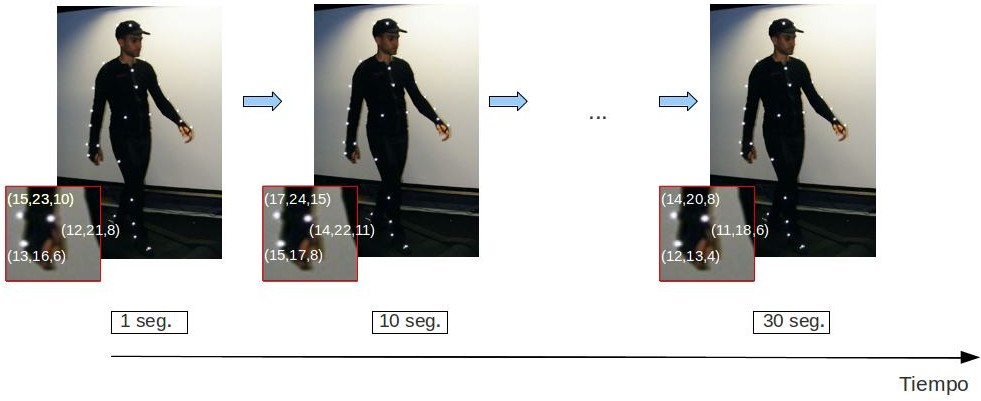
\includegraphics[scale=0.4]{img/Sistema_completo/diagrama_abuelas_2.jpg}
\end{center}
\caption{Posición de los marcadores a lo largo del tiempo.}
\label{abuela2}
\end{figure}

Dicho de otra forma, la aplicación a desarrollar recibe como entrada imágenes de video desde varias cámaras capturando el movimiento de una persona desde distintos ángulos. Dichas cámaras deben estar previamente calibradas. A partir de las imágenes obtenidas se detectan distintos puntos de referencia del cuerpo según el estudio particular que se desee realizar. Este proceso se realiza para cada imagen del video obteniendo así la trayectoria en tres dimensiones de cada punto a lo largo del tiempo. Luego, a partir del procesamiento de la posición 3D de los puntos se obtendrán otros datos estadísticos de interés para el usuario.

\begin{figure}[H]
\begin{center}
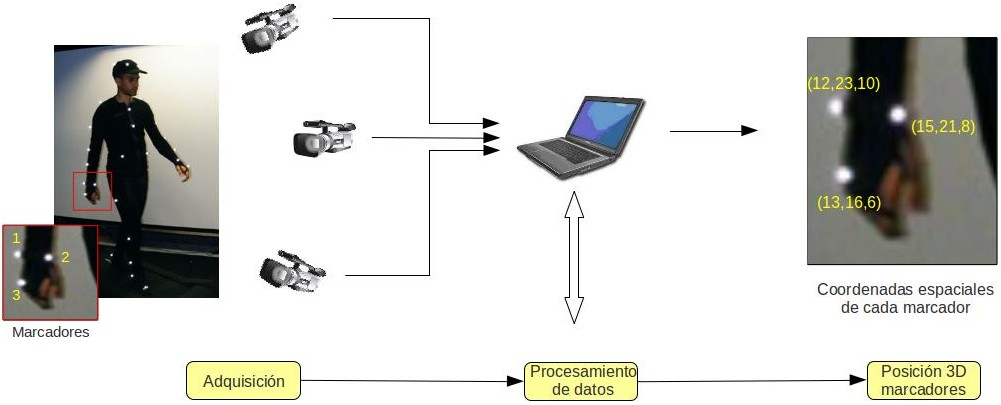
\includegraphics[scale=0.4]{img/Sistema_completo/diagrama_abuelas_1.jpg}
\end{center}
\caption{Funcionamiento de un sistema de captura de movimiento.}
\label{abuela1}
\end{figure}

Los bloques funcionales que debe tener el sistema son:
\begin{itemize}
\item Calibración.
\item Obtención de imágenes de video.
\item Detección y seguimiento de puntos en cada video por separado (posición 2D).
\item Estimación de pose (posición 3D de cada uno de los puntos).
\item Devolución de una matriz de la posición espacial y temporal de los puntos junto con estadísticas generadas a partir de dichos puntos.
\end{itemize}


\subsection{Estado del arte}
%%%%%%%%%%%%%%%%%%%%%%%%%%%%%%%%%%%%%%%%%%%%%%%%%%%%%%%%%%%%%%%%%%%%%%%%%%%%%%%%%%%%%%%%%%%%%%%%%%%%%%%%%%%%%%%%%%%%%%%%%%%%%%%%%%%5
%qué opciones tengo para hacerlo? por qué hay estas opciones? para qué se usan?
%%%%%%%%%%%%%%%%%%%%%%%%%%%%%%%%%%%%%%%%%%%%%%%%%%%%%%%%%%%%%%%%%%%%%%%%%%%%%%%%%%%%%%%%%%%%%%%%%%%%%%%%%%%%%%%%%%%%%%%%%%%%%%%%%%%

A continuación, se hace una breve revisión del estado del arte de los sistemas de caputra de movimiento de las características del que se pretende implementar.

%En relación con esto, se tendrá presente la tecnología del proyecto “Neuronavegador” realizado en Facultad de Ingeniería para obtener puntos contra los cuales comparar los obtenidos por el sistema.

%Dada las características de este proyecto otro antecedente relevante a tener en cuenta en el área, es el de un grupo de investigadores del Hospital de Clínicas que junto al grupo de Tratamiento de Imágenes de la Facultad de Ingeniería han estudiado previamente la marcha de las personas a los efectos de reconocer en ellas patrones de movimiento. Dicho proyecto recibe el nombre “Cíclope”.